% Research Diary Collection Template for Research Student (University), 2025
\documentclass[letterpaper,11pt]{article}
\newcommand{\userName}{Research Student}
\newcommand{\institution}{University}
\newcommand{\workingDate}{2025 Research Diary}
% Modular package loading - choose what you need
% Files are symlinked in output directory for self-contained compilation

\usepackage{assets/styles/diary_base}        % Core packages and basic theorems
\usepackage{assets/styles/diary_theorems}   % Enhanced colored theorem environments
\usepackage{assets/styles/diary_commands}   % Personal shortcuts and commands

\usepackage{tocloft}
\setlength{\cftbeforesecskip}{5pt}
\renewcommand*\contentsname{Research Student's Research Diary -- Contents}

\title{Research Diary Collection - 2025}
\author{Research Student}
\date{Compiled \today}

\begin{document}

\tableofcontents
\thispagestyle{empty}
\newpage


% Entry from 2025-09-20-2.tex
\href{run:2025-09-20-2.tex}{\Huge September 20} %##@@TitleDateString@@##

\section*{Good 2}



\clearpage


% Entry from 2025-09-20-3.tex
\href{run:2025-09-20-3.tex}{\Huge September 20} %##@@TitleDateString@@##

\section*{ }



\clearpage


% Entry from 2025-09-20-best.tex
\href{run:2025-09-20-best.tex}{\Huge September 20} %##@@TitleDateString@@##

\section{It is the best} 



\clearpage


% Entry from 2025-09-20-corrected-test.tex
\href{run:2025-09-20-corrected-test.tex}{\Huge September 20} %##@@TitleDateString@@##

\section*{ }



\clearpage


% Entry from 2025-09-20-newmethod.tex
\href{run:2025-09-20-newmethod.tex}{\Huge September 20} %##@@TitleDateString@@##

\section{New Method}

We have a citation \cite{research_methods2024}.


\clearpage


% Entry from 2025-09-20-test-auto-open.tex
\href{run:2025-09-20-test-auto-open.tex}{\Huge September 20} %##@@TitleDateString@@##

\section{ }



\clearpage


% Entry from 2025-09-20-test-tags.tex
\href{run:2025-09-20-test-tags.tex}{\Huge September 20} %##@@TitleDateString@@##

\section*{ }



\clearpage


% Entry from 2025-09-20.tex
\href{run:2025-09-20.tex}{\Huge September 20} %##@@TitleDateString@@##

\section*{Reflow}

\begin{figure}[h]
\centering 
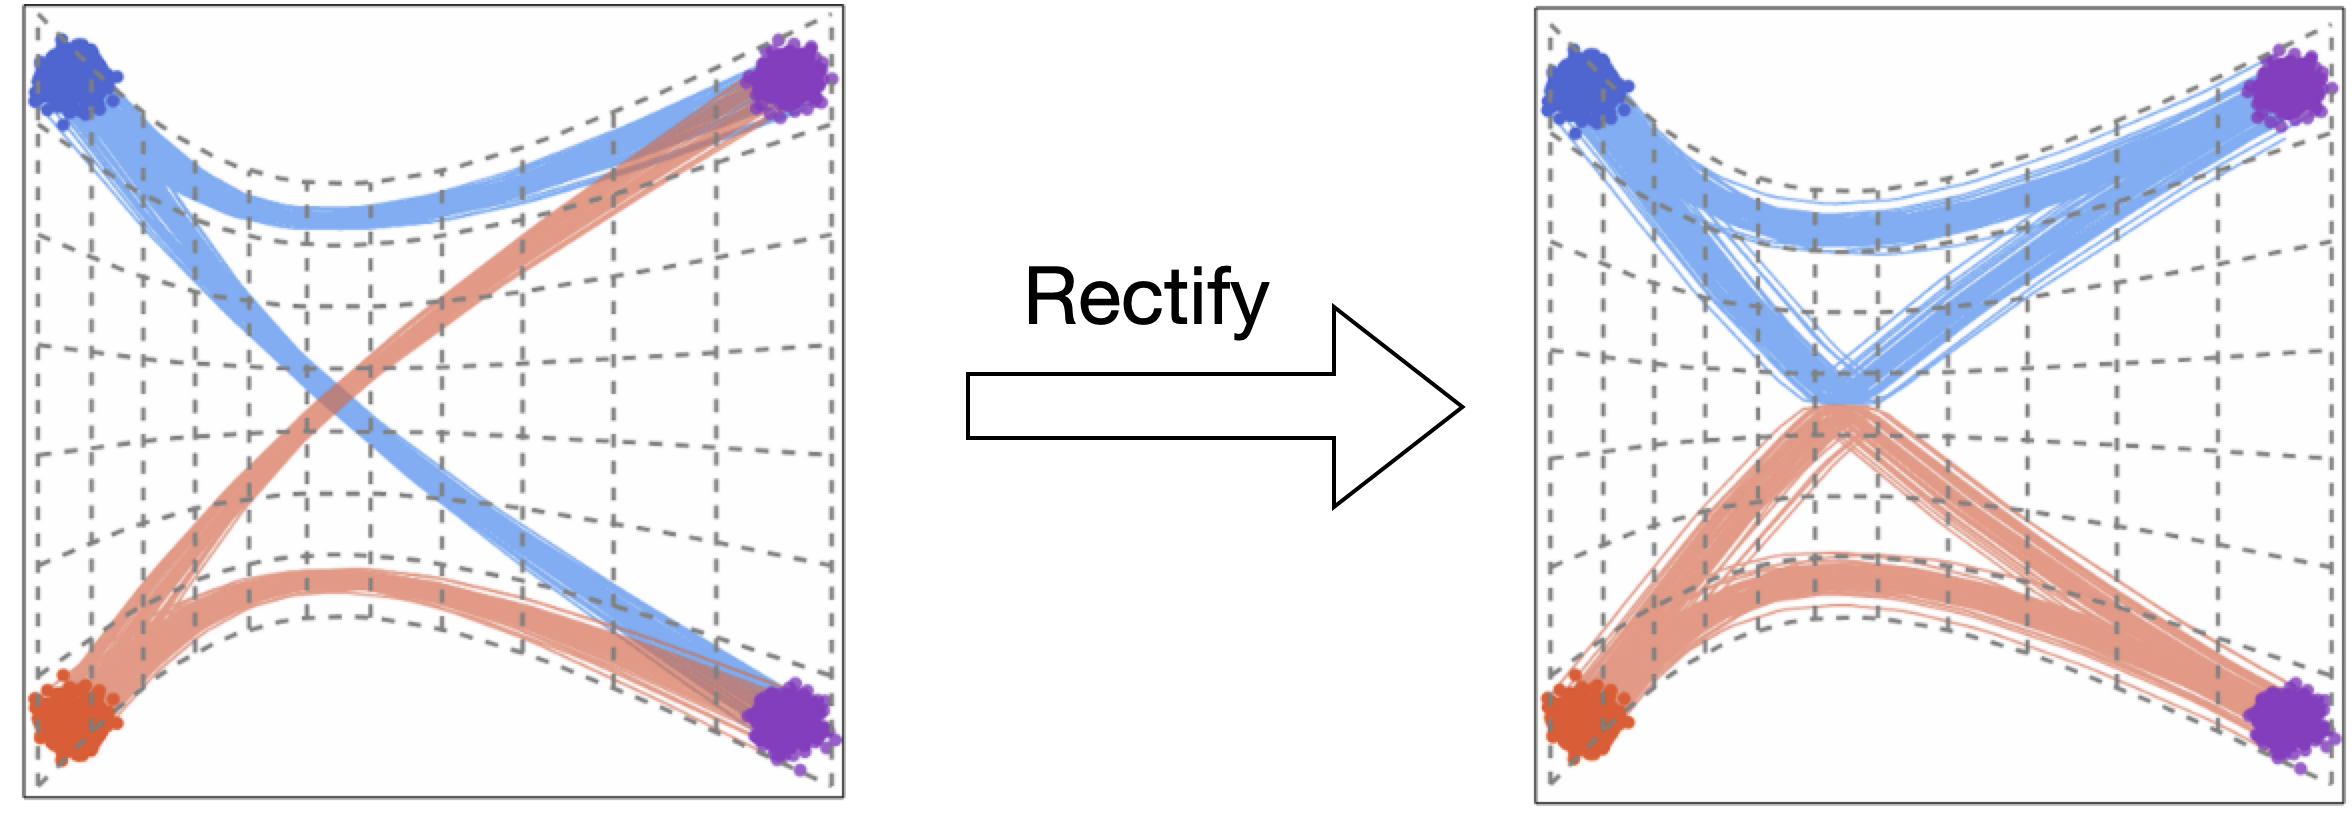
\includegraphics[width=0.8\textwidth]{assets/figures/2025/curved_reflow.png}
\end{figure} 


Yes. I want to cite \cite{li2022diffusion}. 



\clearpage


\bibliographystyle{apalike}
\bibliography{assets/bibliography/reference,assets/bibliography/z}


\end{document}
